\chapter{Results}

\section{Neural networks performance}
For the correct functionality of the algorithm, it is required that the network is able to recognize the shapes. There are numerous parameters for the neural networks, like the training algorithm choice, architecture, activation function. Because it is not feasible to test every combination of the parameters, we have tested the influence of only a several of these parameters, with the following set up:
\begin{description}
\item [Network architecture] The networks had a layered structure, with two hidden layers.
\item [Training algorithm] resilient back-propagation, alias rprop.
\item [Activation function] The Elliot activation function, faster version of the sigmoid activation function, which is considered a standard used in most applications.
\item [Shape descriptors] We have used four basic shapes: square, circle, triangle, a water drop. 
\item [Data] The training data and the test data were generated by the developed generator. The training data consisted of 150 000 images with some shape, each shape had the same amount of examples and 50 000 images of random data without shape pattern. The test data consisted of 40 000 images of examples of shapes, and 20 000 images of random data.
\end{description}

The parameters that we have tested are these:
\begin{description}
\item [Number of neurons] We have tried several values of both layers. For the first hidden layer, we have tried 100, 200 and 300 neurons, and for the second hidden layer 10, 20 and 30 neurons. 
\item [The value of MSE] We have trained the networks at different levels of precision, with the target MSE values of 0.1, 0.07, 0.04 and 0.01.   
\item [Algorithm settings] The neural networks were trained for different combinations of algorithm settings, with embeddings and composition off and on.
\end{description}
The combinations of the parameters above gave us 3*3*4*4 = 150 trained neural networks to evaluate.

\section{Evaluation}
The networks were evaluated in the following scenario. For each of the combinations of embeddings and composition being turned on or off, the dataset of 1000 images were generated, with the same amount of examples for each shape. Then, the network was assigned a score computed as a sum of scores for each example. Score per example was one of following:

\begin{description}
\item [1] If the maximum of the outputs of the network is in the corresponding output neuron of the shape that is in the example.
\item [2] If the maximum of in the correct output neuron and is higher than 0.5.
\item [-1] If the maximum is in the wrong output neuron which corresponds to the different shape than the one in the image.
\end{description}

These rules mimic the usage of the network in the algorithm, where value above 0.5 is a match and only maximum is considered. From the rules follows, that each network could achieve from -1000 to 2000 score points. 

\section{Algorithm parameters optimization}
Plot in \cref{fig:simples_com} shows the measurements of algorithm performance for various parameters, as described in the legend. \todo{nasledujici patri do captionu toho figure! misto toho by chtelo rict co ten vysledek vlastne znamena --- napr. zjistili jsme ze je neco optimalni nebo ze neco se vylozene nehodi?}The X-axis represents score, the Y-axis represents final MSE of the network in training and each object represents a single network, with training parameters as described in the legend.

\todo{exportovat grafy jako pdf}
\todo{lepe popsat co v tom grafu je}
\begin{figure}
\centering
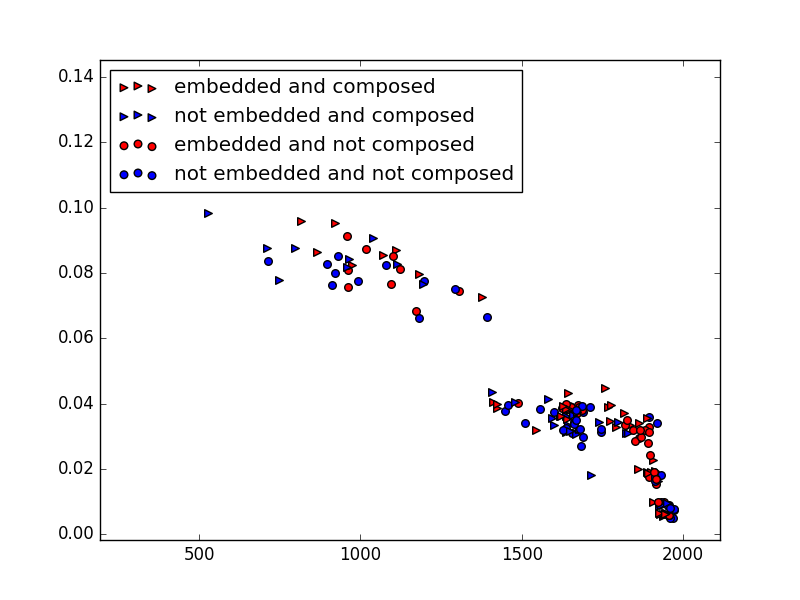
\includegraphics[width=.8\linewidth]{ext/figure_simples_com.png}
\caption{scores on data with simple shapes only, no embeddings and no composition}
\label{fig:simples_com}
\end{figure}

\begin{figure}
\centering
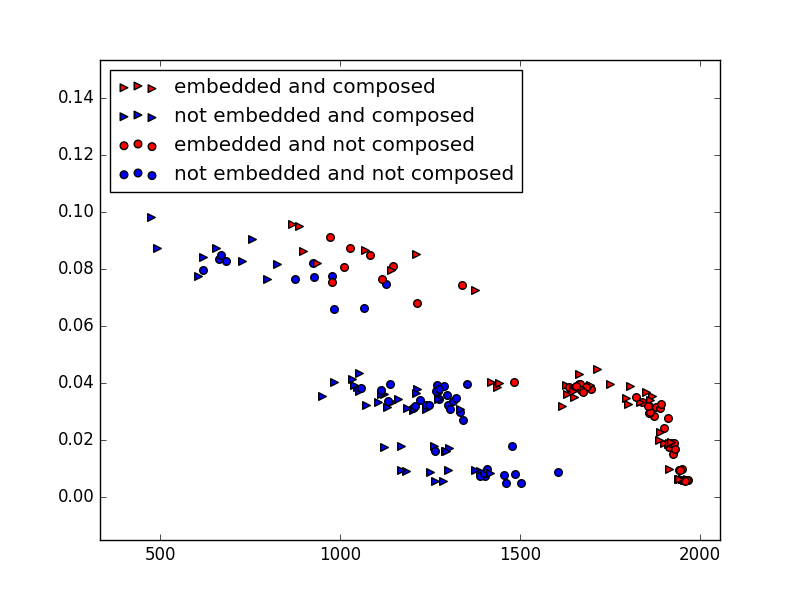
\includegraphics[width=.8\linewidth]{ext/figure_embed_com.png}
\caption{Scores on data with embeddings, no composition}
\label{fig:embed_com}
\end{figure}


\begin{figure}
\centering
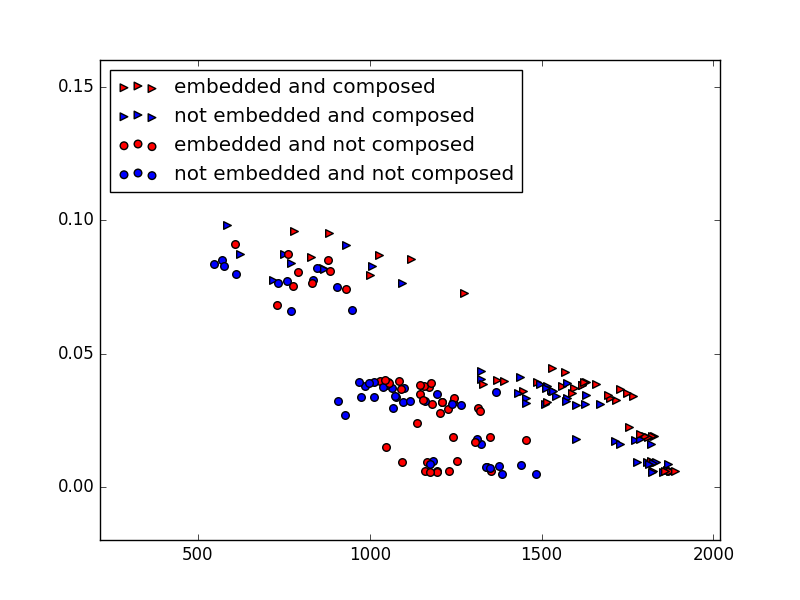
\includegraphics[width=.8\linewidth]{ext/figure_comp_com.png}
\caption{Scores on data with composition, no embeddings}
\label{fig:comp_com}
\end{figure}


\begin{figure}
\centering
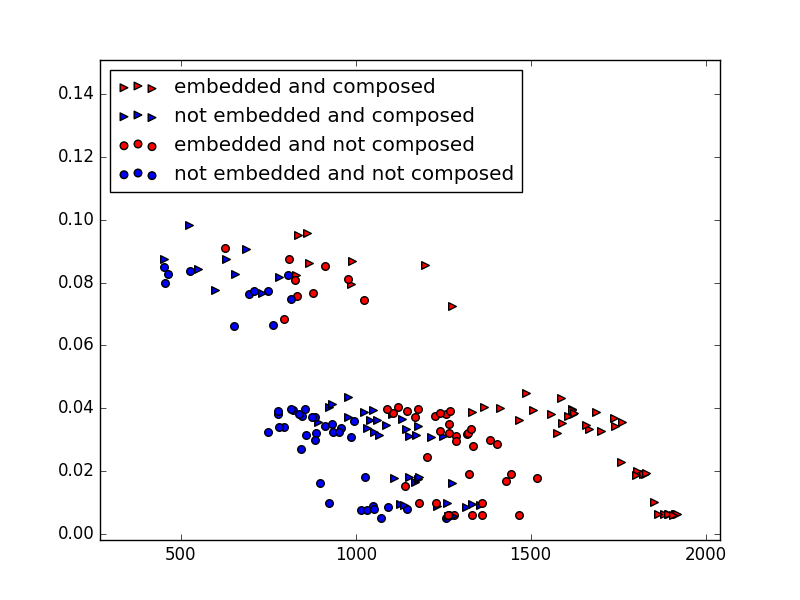
\includegraphics[width=.8\linewidth]{ext/figure_x_com.png}
\caption{Scores on data with both embeddings and composition combined}
\label{fig:x_com}
\end{figure}

From the \cref{fig:comp_com} \todo{it} is clear, that it is important to train the network for combinations of both embeddings and composition. More interesting is the observation from \cref{fig:simples_com} that turning on embeddings and composition affects the recognition of the simple shapes very slightly when reaching very low MSE. From the figures, it can also be observed, that the tendency to overtrain is not present and it is preferable to aim for lower MSE values in training.

\section{Network architecture}
\todo{opet: influence of the network architecture}
\Cref{fig:simples_arch,fig:embed_arch,fig:comp_arch,fig:x_arch} \todo{vsechny obrazky musi mit odkaz z textu, jinak ctenare nic nenuti na ne vubec kouknout :D} show the influence of different layer sizes on the overall performance of the network. Again, the X-axis represents score, the Y-axis represents final MSE of the network in the training and each object represents a single network, with the architecture described in the legend. Color represents the size of the first hidden layer, while shape represents the size of the second hidden layer.

\begin{figure}
\centering
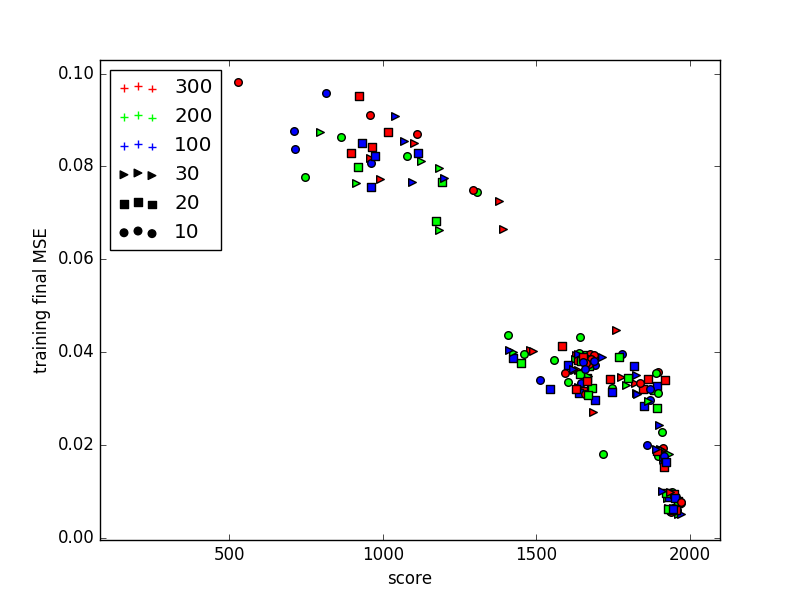
\includegraphics[width=.8\linewidth]{ext/figure_simples_arch.png}
\caption{scores on data with simple shapes only, no embeddings and no composition}
\label{fig:simples_arch}
\end{figure}

\begin{figure}
\centering
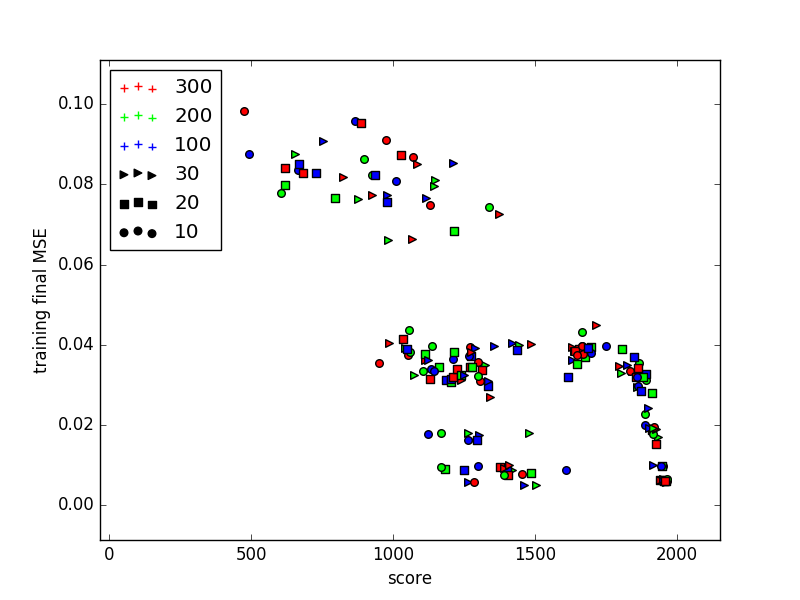
\includegraphics[width=.8\linewidth]{ext/figure_embed_arch.png}
\caption{Scores on data with embeddings, no composition}
\label{fig:embed_arch}
\end{figure}

\begin{figure}
\centering
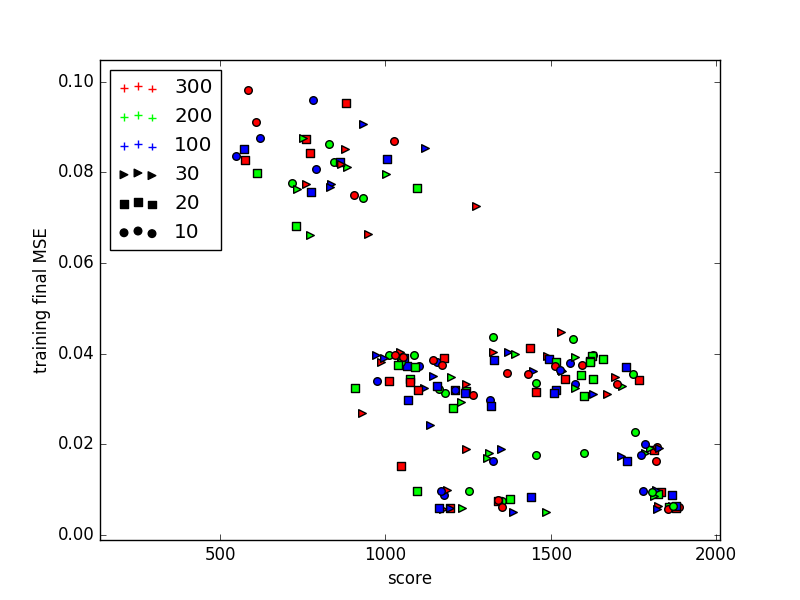
\includegraphics[width=.8\linewidth]{ext/figure_comp_arch.png}
\caption{Scores on data with composition, no embeddings}
\label{fig:comp_arch}
\end{figure}

\begin{figure}
\centering
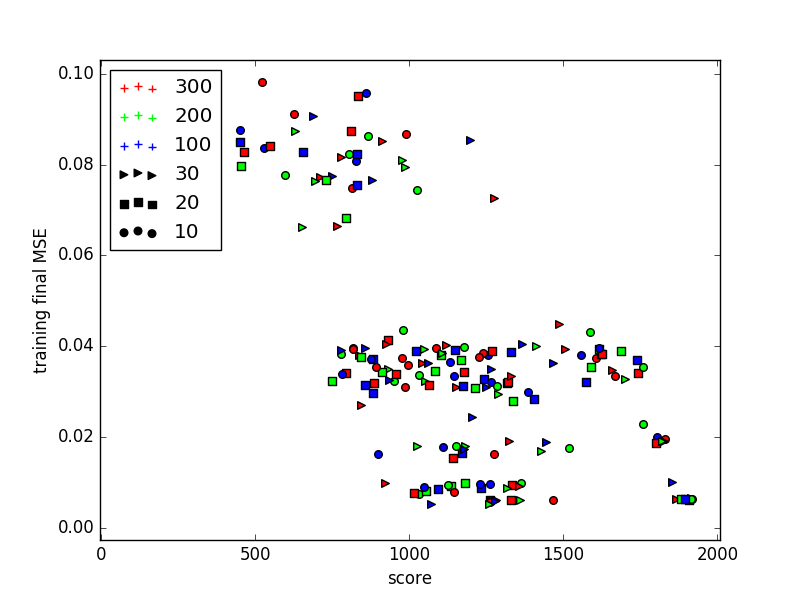
\includegraphics[width=.8\linewidth]{ext/figure_x_arch.png}
\caption{Scores on data with both embeddings and composition combined}
\label{fig:x_arch}
\end{figure}

The figures do not show any clear pattern. All the values used in the tests were able to achieve good results, even the network with the lowest number of neurons. It may be necessary to increase the number for a higher count of shape descriptors, but for the four used shape descriptors, even the 100-10 network was sufficient.

\section{Composition recognition}
To measure composition precision, we have prepared 100 \emph{ImageLines} instances of composition examples. Each instance represented a shape composed of examples of another shape. In the algorithm, we have used the best performing network trained for both composition and embeddings. Then we have analyzed the instances under the following set up:
\begin{enumerate}
\item \texttt{COMPOSED\_SHAPES\_ENABLED = true;}
\item \texttt{EMBEDDED\_SHAPES\_ENABLED = false;}
\item \texttt{ROTATION\_ENABLED = false;}
\end{enumerate}

\todo{tady odsud by to ty identifikatory chtelo vsechno dat do texttt}

We have tested different combinations of settings of variables COMPOSITION\_SAMPLES\_COUNT, COMPOSITION\_SAMPLES\_LIMIT and COMPOSITION\_WINDOW\_SIZE. We have compared the correct pattern shape with the recognized pattern shape for each test instance. The Y-axis shows the percentage of correct pattern shape recognitions and the X-axis shows a count of samples made around the shape contour. In \cref{fig:com,fig:com_speed} the COMPOSITION\_WINDOW\_SIZE is represented by the color and the COMPOSITION\_SAMPLES\_LIMIT by the shape. The COMPOSITION\_SAMPLES\_COUNT is on the X-axis. 
\begin{figure}
\centering
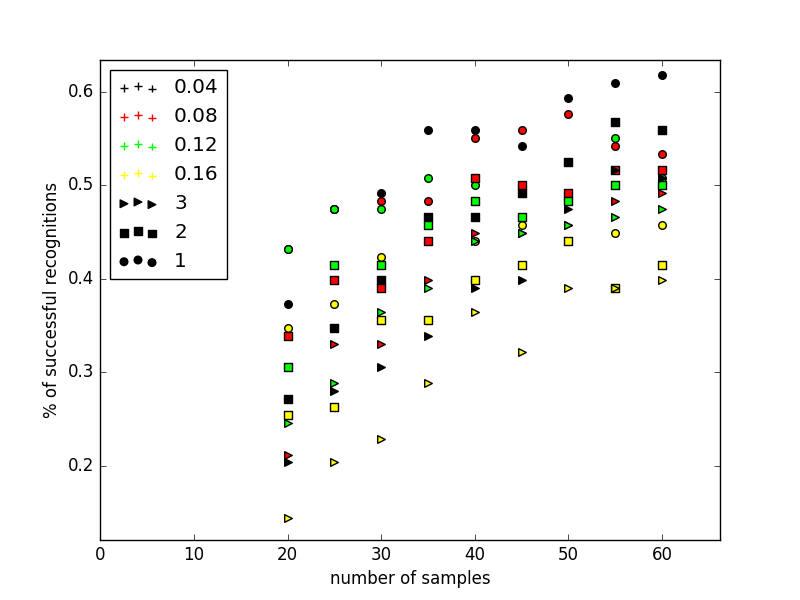
\includegraphics[width=.8\linewidth]{ext/figure_composition.png}
\caption{Precision of composition recognition. \XX{Jsou tady na ty ose Y fakt procenta? jestli jo tak 0.5\% neni vubec moc. :D}}
\label{fig:com}
\end{figure}

In \cref{fig:com}, we can see that success rate grows with the increasing number of samples. We can also see that the red and black colors representing the smaller sizes of the sample window perform better with the higher sample count. There is also a great drop in success rate when increasing the sample limit even by one. There are several factors that affect the recognition. The sampling window follows the ideal path from the shape descriptor, but the real shape is usually more or less deformed, which means that the window will hit only a part of the pattern shape. The pattern shapes can be of various sizes which is hard to approximate by the single size of the sampling window. And even the window hits the whole pattern shape, there is a very high chance of hitting also the noise from other shape patterns, or from embeddings. All these factors make the recognition for the network very difficult. From the shape locations in \cref{fig:com} we can deduce that the network is rarely able to recognize even a single pattern shape correctly, and after 40 samples, the success rate does not improve much and stays somewhere between 40\% and 60\%.

\begin{figure}[!htb]
\centering
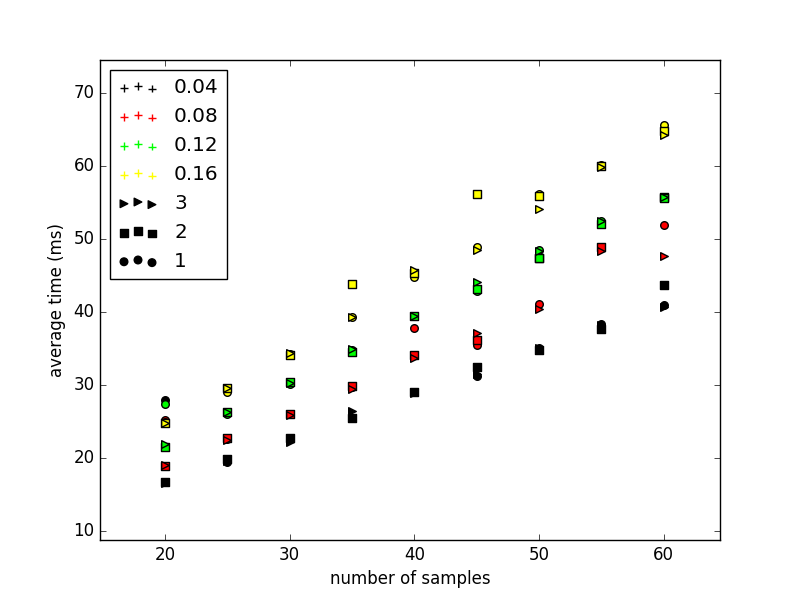
\includegraphics[width=.8\linewidth]{ext/figure_composition_speed.png}
\caption{Performance of composition recognition}
\label{fig:com_speed}
\end{figure}

It is clear that the algorithm becomes gradually slower with the increasing number of samples as shown in \cref{fig:com_speed}. The total time will also increase substantially if the rotation is turned on.

\section{Rotation}
Rotation invariance is achieved by redrawing the image at different angles and returning the best match from all samples [TODO ref description]. We tested the influence of the ROTATION\_SAMPLES\_COUNT on the precision and speed of the algorithm. In \cref{fig:rotation_simple_precision} we can see that the precision reaches a very high success rate at 15 samples and the computation time is linear to samples count and \todo{and what?} \cref{fig:rotation_simple_speed}. However, the performance of rotation recognition on composed shapes is much worse both in precision and computation time. From \cref{fig:rotation_comp_precision} we can see that the precision reaches about 70\% at 15 samples and improves only a little when we increase the samples count. The speed of recognition of composed shapes is slower by a magnitude in \cref{fig:rotation_comp_speed}. This is caused by the fact, that composed shapes contain a lot more lines than the simple shapes. We can deduce that setting ROTATION\_SAMPLES\_COUNT to higher than 15 is rather impractical.

\begin{figure}
\centering
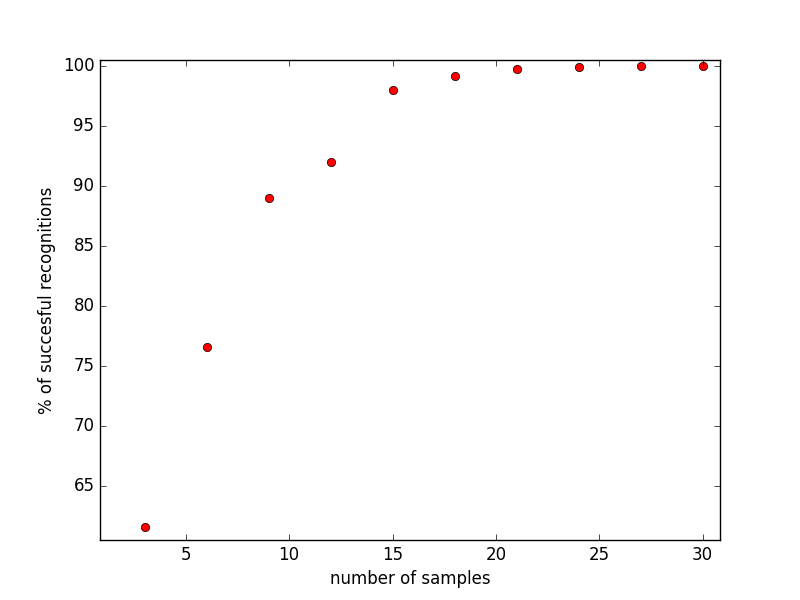
\includegraphics[width=.8\linewidth]{ext/rotation_simple_precision.png}
\caption{Precision of rotation recognition of simple shapes}
\label{fig:rotation_simple_precision}
\end{figure}

\begin{figure}
\centering
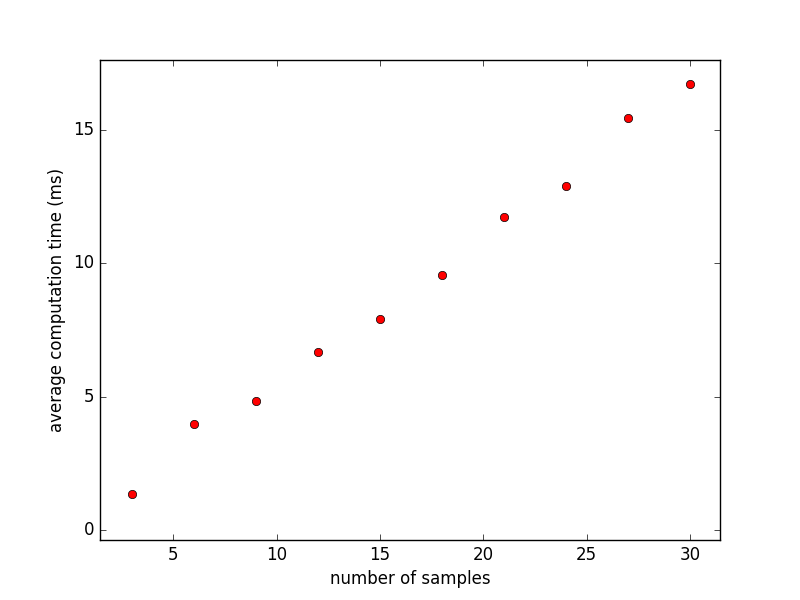
\includegraphics[width=.8\linewidth]{ext/rotation_simple_speed.png}
\caption{Performance of rotation recognition of simple shapes}
\label{fig:rotation_simple_speed}
\end{figure}

\begin{figure}
\centering
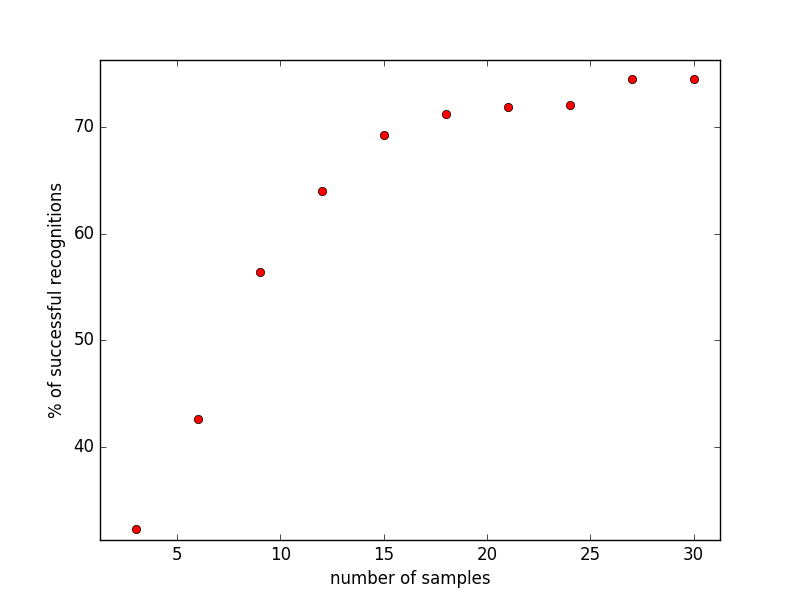
\includegraphics[width=.8\linewidth]{ext/rotation_comp_precision.png}
\caption{Precision of rotation recognition of composed shapes}
\label{fig:rotation_comp_precision}
\end{figure}

\begin{figure}
\centering
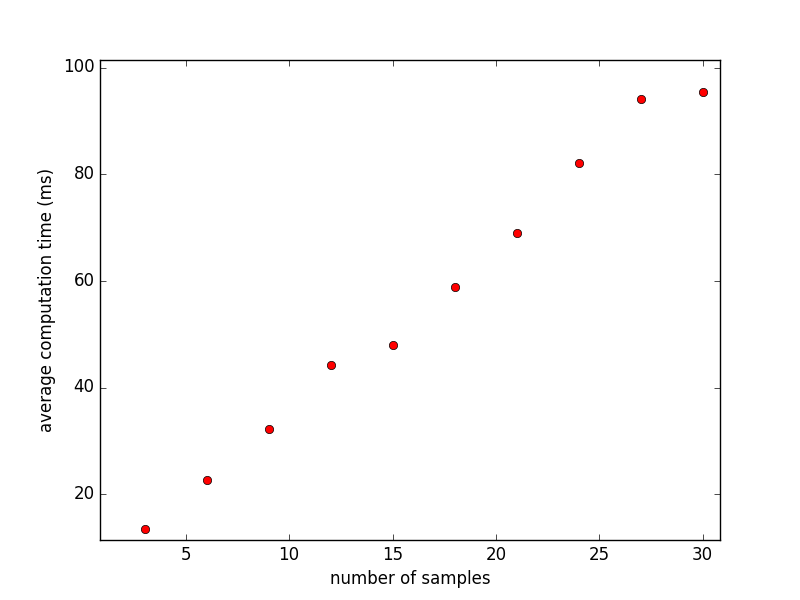
\includegraphics[width=.8\linewidth]{ext/rotation_comp_speed.png}
\caption{Performance of rotation recognition of composed shapes}
\label{fig:rotation_comp_speed}
\end{figure}

\section{Embeddings}
The ability of the algorithm to recognize embeddings depends on the shape descriptor definition. There the user can define the points of interest by their position and size. These two parameters form a rectangular area where the algorithm will search for embedded shape. It is then recommended to set the size of this area lower, to avoid fragments of the top shape appearing in this area, which might cause the network to not recognize the embedded shape. If the embeddings should appear in the composed shapes, the area should be even smaller, otherwise, the fragments of the pattern shapes will appear inside. The speed is influenced by the number of embeddings such that every point of interest if analyzed recursively.

\todo{Chces sem dat nekolik screenshotu ze hry ktery demonstrujou jak to nakonec vypada. Zaroven by nebylo spatny ukazat nejakej malej sample tech trenovacich a generovanejch dat, pripadne nejaky outliery (ty sou vzdycky zajimavy). Obecne by hodne prospel i zajimavej obrazek toho co presne vizualne znamena embedding a composition, hned k zacatku tyhle kapitoly.}
\todo{Diskusion jen pokud je potreba, jinak je to uz popsane vyse}
